\chapter{Experiments}

The goal of the experiment is to compare the training and test performance of GIN and (less powerful) GNN variants.\footnote{The code is available at \url{https://github.com/weihua916/powerful-gnns}}
Specifically,

\begin{itemize}
	\item Training set performance: compare different GNN models based on their {\it representational power}

	\item Test set performance: quantifies {\it generalization ability}
\end{itemize}

\section{Experiment Design}

9 graph classification benchmarks\cite{Yanardag2015} were used:

\begin{itemize}
	\item 4 bioinformatics datasets: MUTAG, PTC, NCI1, PROTEINS
	\item 5 social network datasets: COLLAB, IMDB-BINARY, IMDB-MULTI, REDDIT-BINARY, REDDIT-MULTI5K
\end{itemize}

The authors have preprocessed some of the datasets.
The nodes of bioinformatics datasets already have categorical input features, so they were left untouched.
Social network datasets, on the other hand, have no node features. To not allow the models to rely on the input node features but mainly learn from the network structure, the authors have created the node features for the social network datasets as follows: for the REDDIT datasets, all node feature vectors were set to be the same; for the other social graphs, one-hot encodings of node degrees were used.

Several models were used:
\begin{itemize}
	\item $\gin-\epsilon$: $\gin$ that {\it learns} $\epsilon$ by gradient descent
	\item $\gin-0$: $\gin$ that fixes $\epsilon$ to $0$.
	\item Architectures that replace the sum in the $\gin-0$ aggregation with mean or max-pooling, or replace MLPs with 1-layer perceptrons
	\item GCN
	\item GraphSAGE
\end{itemize}
(There exists some contrived graphs that $\gin-\epsilon$ can distinguish but $\gin$ cannot.)
(Specific choices of hyperparameters are omitted in this writing. Curious readers may refer to the original paper\cite{Wu2019}.)

Baselines that were used:

\begin{itemize}
	\item WL subtree kernel with $C$-SVM used as a classifier
	\item Deep learning architectures i.e. DCNN, PATCHY-SAN, DGCNN
	\item AWL
\end{itemize}

\section{Results / Analysis}

\subsection{Training set performance}

\begin{figure}[!hbt]
  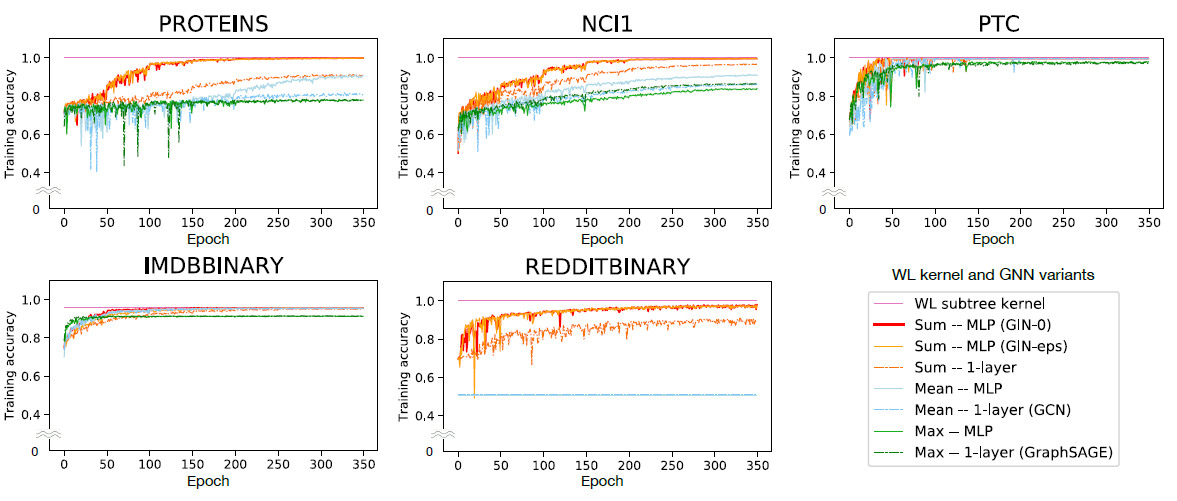
\includegraphics[height=7cm]{experiments/fig/fig5.png}
  \caption{Training set performance}
\end{figure}

%It is obvious that models with higher representational power should have higher training set accuracy.
Above figure shows the training curves of GINs and less powerful GNN variants with the same hyper-parameter settings.

First, observe that both the theoretically most powerful GNN, i.e. $\gin-\epsilon$ and $\gin-0$, are able to almost perfectly fit all the training sets.
In comparison, the GNN variants using mean/max pooling or 1-layer perceptrons severely underfit on many datasets.
This shows that the training accuracy patterns align with the ranking of the models’ representational power.
%: GNN variants with MLPs tend to have higher training accuracies than those with 1-layer perceptrons, and GNNs with sum aggregators tend to fit the training sets better than those with mean and max-pooling aggregators.

Also, the training accuracies of the GNNs never exceed those of the WL subtree kernel. This aligns with the result that the WL test provides an upper bound for the representational capacity of the aggregation-based GNNs.

One particular interesting observation is that the explicit learning of $\epsilon$ in $\gin-\epsilon$ yielded no gain in fitting training data compared to $\gin-0$, where $\epsilon$ is fixed to $0$.



\subsection{Test set performance}

\begin{figure}[!hbt]
  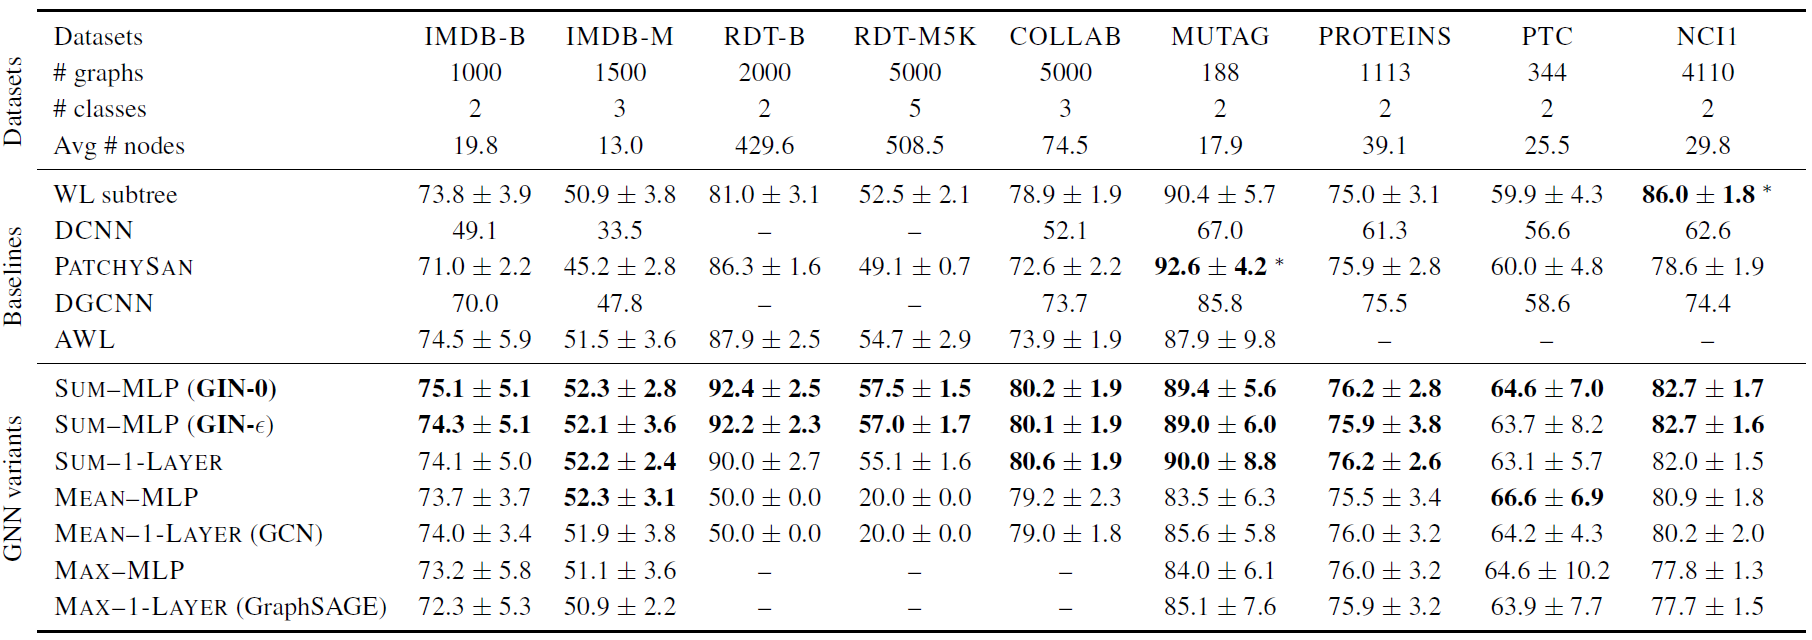
\includegraphics[height=6cm]{experiments/fig/fig6.png}
  \caption{Test set performance}
\end{figure}

%Although the authors' theoretical results do not directly speak about the generalization ability of GNNs, it is reasonable to expect that GNNs with strong expressive power can accurately capture graph structures of interest and thus generalize well.
Above table compares the test accuracies of GINs (Sum–MLP), other GNN variants, as well as the state-of-the-art baselines.

First, GINs, especially $\gin-0$, outperform the less powerful GNN variants on all the 9 datasets, achieving state-of-the-art performance.

In the Reddit datasets, where all nodes share the same scalar as node feature, GINs and sum-aggregation GNNs accurately capture the graph structure and significantly outperform other models.
Mean-aggregation GNNs, however, fail to capture any structures of the unlabeled graphs and do not perform better than random guessing.
(The same phenomenon is observed when the node degrees are provided as input features.)
This, again, aligns with the ranking of the models’ representational power, based on its aggregator.

One interesting observation here is that $\gin-0$ slightly but consistently outperforms $\gin-\epsilon$. The authors explain this better generalization by arguing that the model complexity of $\gin-\epsilon$ is higher than $\gin-0$. This has not been theoretically confirmed, though.

One might ask why WL subtree kernel doesn't act as an upper bound as it did in the training set performance. This can be explained by the fact that WL kernel, unlike the GINs, can't learn how to combine node features, which might be quite informative for a given prediction task.


\section{Remark}

Note that the authors have not performed experiments regarding node classification. As they've stated in \url{https://openreview.net/forum?id=ryGs6iA5Km}, there are two reasons of why they didn't do that.

Borrowing their words,

\begin{enumerate}
\item In many node classification applications, node features are rich and diverse (e.g. bag-of-words representation of papers in a citation network), so GNN models like GCN and GraphSAGE are often already able to fit the training data well.

\item Many node classification tasks assume limited training labels (semi-supervised learning scenario); thus, the inductive bias of GNNs also plays a key role in empirical performance. For example, the statistical and distributional information of neighborhood features may provide a strong signal for many node classification tasks.
\end{enumerate}

It may be the case that GIN performs well on node classification tasks. However the performance on node classification tasks are less directly explained by the authors' theory of representational power, which is why the authors have left that part out.